\section{Evaluation}

\subsection{Data}

WODA was deployed to address OLAF for a specific geographic sample, that is the same five OS 1:10,000 raster tiles that were previously used in literature to analyse the performance of GI crowdsourcing and originally selected by Haklay in \cite{Haklay:2010vs} to assess OSM\footnote{The tiles are: TQ37ne, TQ28ne, TQ29nw, TQ26se and TQ36nw.}.

Figure \ref{fig:scope} shows the sample in the context of the overall OLAF problem for the UK. The scope is large enough to be relevant, covering an area of ~113 $ km^2 $ of Greater London that includes 3,982 roads\footnote{Roads were considered in scope if they are classified by OSON as "named roads" and are fully included within any of the five tiles.}. At the same time, it is small enough not to be "big data", and was manageable using conventional data processing tools, e.g. manual visual verification for debugging. Because of London's long and complex history, the city offers a worst case scenario for evaluation, as the shape of the streets is not trivial, they have been subject to a lot of development over time etc. 

\subsection{Ingestion of primary data sources}

The data obtained by implementing the approach described in section \ref{crowdsourcing-olaf} successfully populated house numbers from LRPP for 82\% of the streets in OSON.

\subsection{House number inference}

The conditions necessary to apply the inference algorithms, before using any crowdsourcing, were verified for 74\% of roads. Applied to these, algorithms \ref{algo:inference-numbers} and \ref{algo:inference-numbers-suffix} generated ~113k house numbers in addition to the already known ~111k. Figure \ref{fig:results-inference} summarises these results.

\begin{figure}[!ht]
    \begin{floatrow}
        \ffigbox{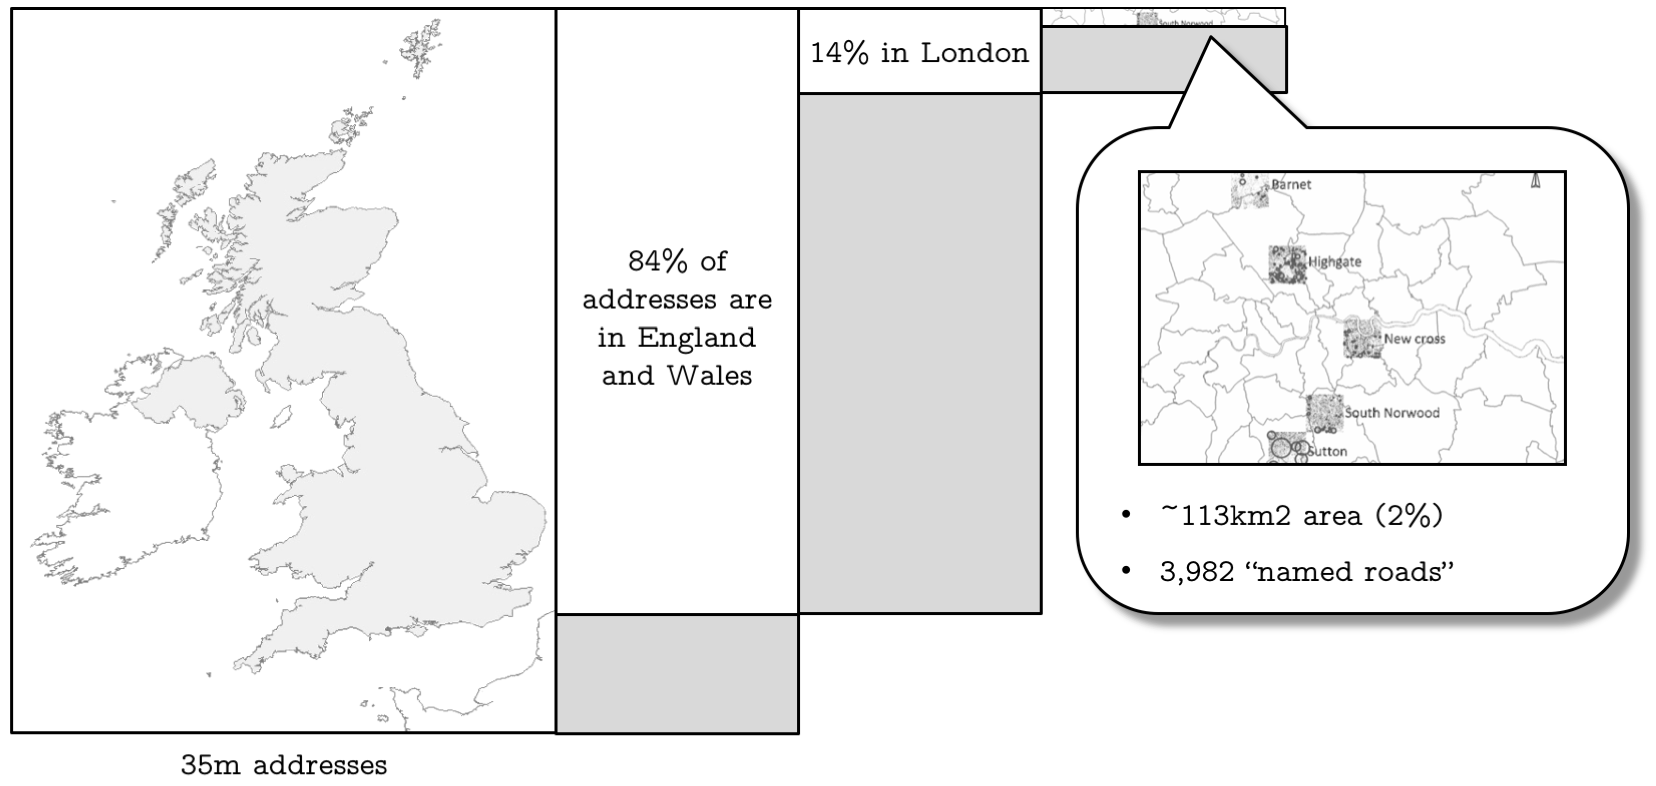
\includegraphics[width=0.505\textwidth]{scope.png}}{\caption{Scope for the evaluation. Figures are estimates derived from the UK Census 2011.}\label{fig:scope}}
        \ffigbox{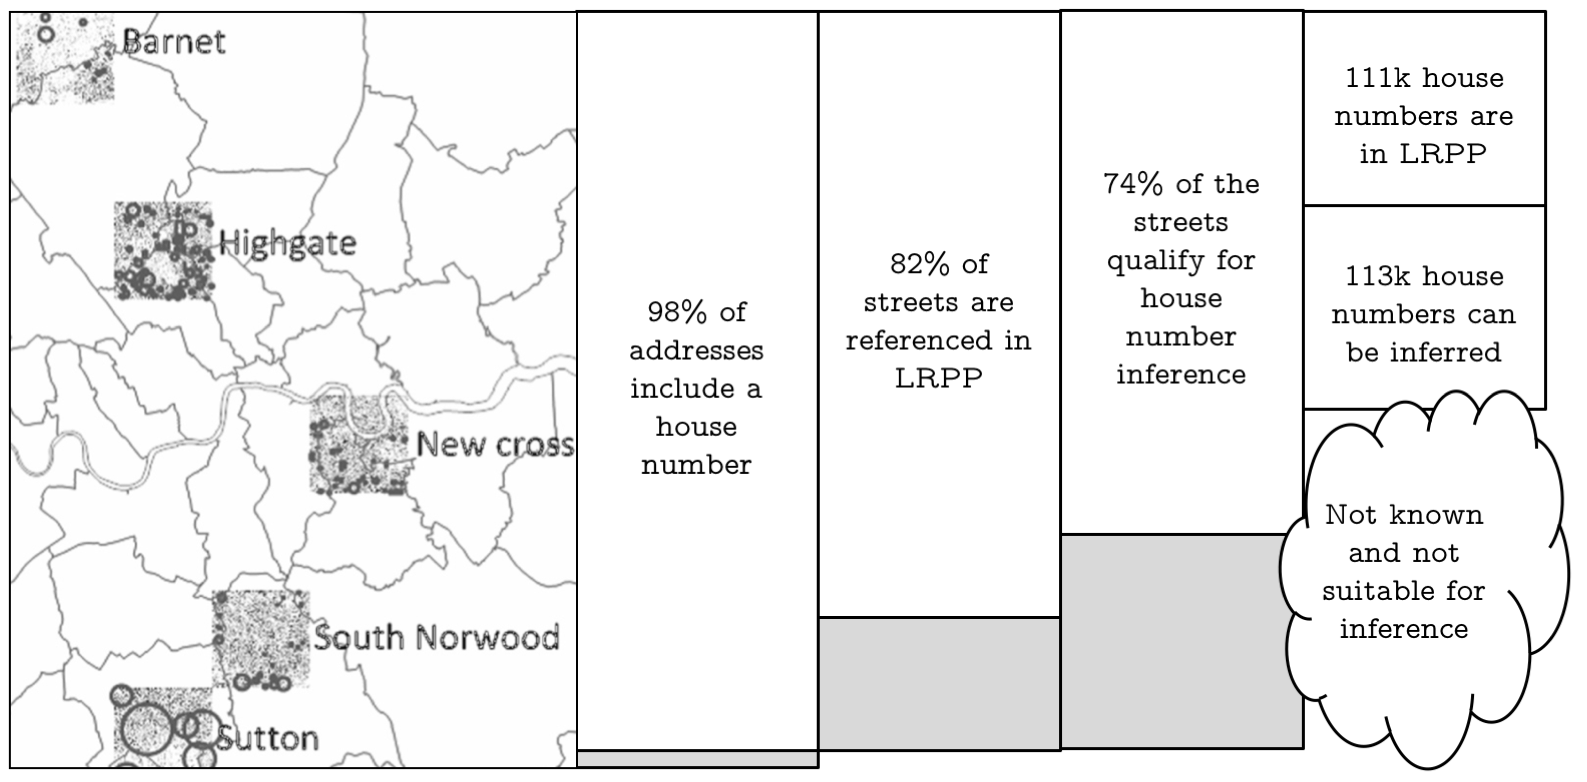
\includegraphics[width=0.475\textwidth]{inference-results.png}}{\caption{Results summary of ingestion and inference.}\label{fig:results-inference}}
   \end{floatrow}
\end{figure}

\subsection{House number crowdsourcing}

The result of the crowdsourcing experiments is summarised in tables \ref{table:distribution-of-workers} and \ref{table:judgements-summary}. 

A significant volume of Workers, 18.75\%, failed the test of copying the name of the road in the form and thus were identified as not credible. Their contribution was ignored.

Three rounds of 10 judgements per road were required to reach any consensus on the first batch of roads published on CrowdFlower. The judgements of 65 credible workers identified 4 out of the 10 roads as not having house numbers.

Those three rounds were sufficient to hit one of the stop conditions: the total number of duplicate judgements by credible Workers was higher than the number of unique judgements, 118 vs 117.

Three additional rounds were run at a later point in time to attempt leveraging a different Worker base. The judgements of 41 additional Workers were collected, achieving consensus on 3 more roads. The volume of duplicates,  73.1\% of total, was well beyond acceptable to keep the experiment going at that stage.

\begin{table}[]
\centering
\begin{tabular}{|l|c|c|l|l|l|}
\hline
                   & \multicolumn{1}{l|}{\begin{tabular}[c]{@{}l@{}}Tot. no. of \\ Workers\end{tabular}} & \multicolumn{1}{l|}{\begin{tabular}[c]{@{}l@{}}No. of new \\ Workers\end{tabular}} & \begin{tabular}[c]{@{}l@{}}No. of \\ credible\\ Workers\end{tabular} & \begin{tabular}[c]{@{}l@{}}\% of \\ credible \\ Workers\end{tabular} & \begin{tabular}[c]{@{}l@{}}\% of duplicate \\ judgements\end{tabular} \\ \hline
First three rounds & 80                                                                                  & -                                                                                  & 65                                                                   & 81.25\%                                                              & 50.2\%                                                                \\ \hline
All six rounds     & 121                                                                                 & 41                                                                                 & 97                                                                   & 80.16\%                                                              & 73.1\%                                                                \\ \hline
\end{tabular}
\caption{Distribution of Workers across rounds}
\label{table:distribution-of-workers}
\end{table}

\begin{table}[]
\centering
\begin{tabular}{|l|l|l|l|}
\hline
                   & \begin{tabular}[c]{@{}l@{}}No. of \\ reliable\\ Workers\end{tabular} & \begin{tabular}[c]{@{}l@{}}No. of non-duplicate\\ judgements\end{tabular} & \begin{tabular}[c]{@{}l@{}}No. of roads\\ where consensus\\ was achieved\end{tabular} \\ \hline
First three rounds & 65                                                                   & 117                                                                       & 4                                                                                     \\ \hline
All six rounds     & 97                                                                   & 227                                                                       & 7                                                                                     \\ \hline
\end{tabular}
\caption{Judgement numbers and consensus summary}
\label{table:judgements-summary}
\end{table}

Diagrams \ref{fig:results-lowest-not-found} to \ref{fig:results-highest-found} show the evolution of the measure of Worker consensus through iterations, in the attempt to identify a trend. 

\begin{figure}[!ht]
    \begin{floatrow}
        \ffigbox{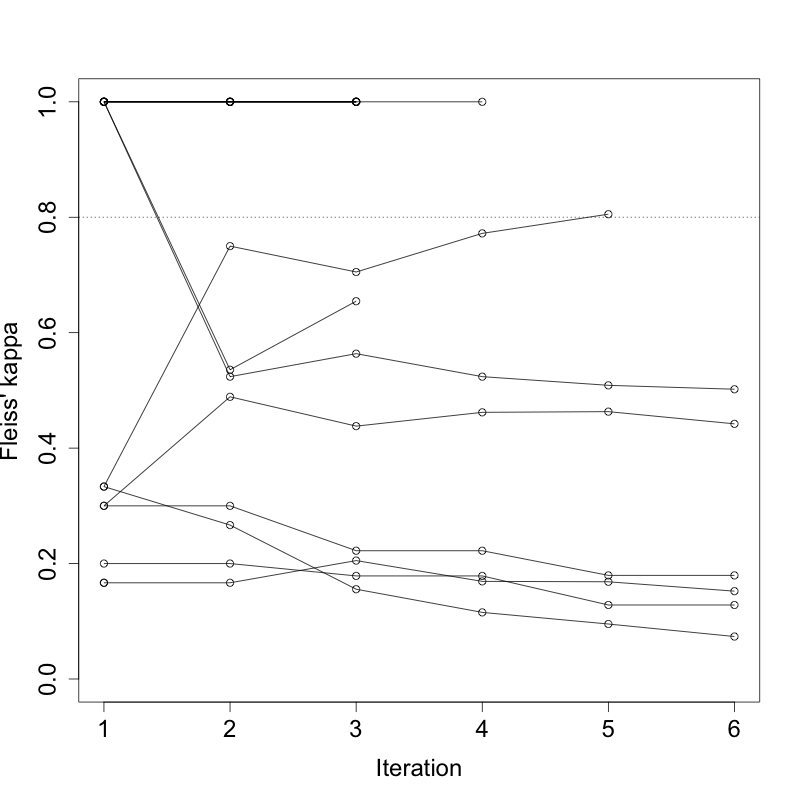
\includegraphics[width=0.49\textwidth]{results-lowest-not-found.png}}{\caption{Roads for which the house numbers were not found. Submissions for the lowest house number.}\label{fig:results-lowest-not-found}}
        \ffigbox{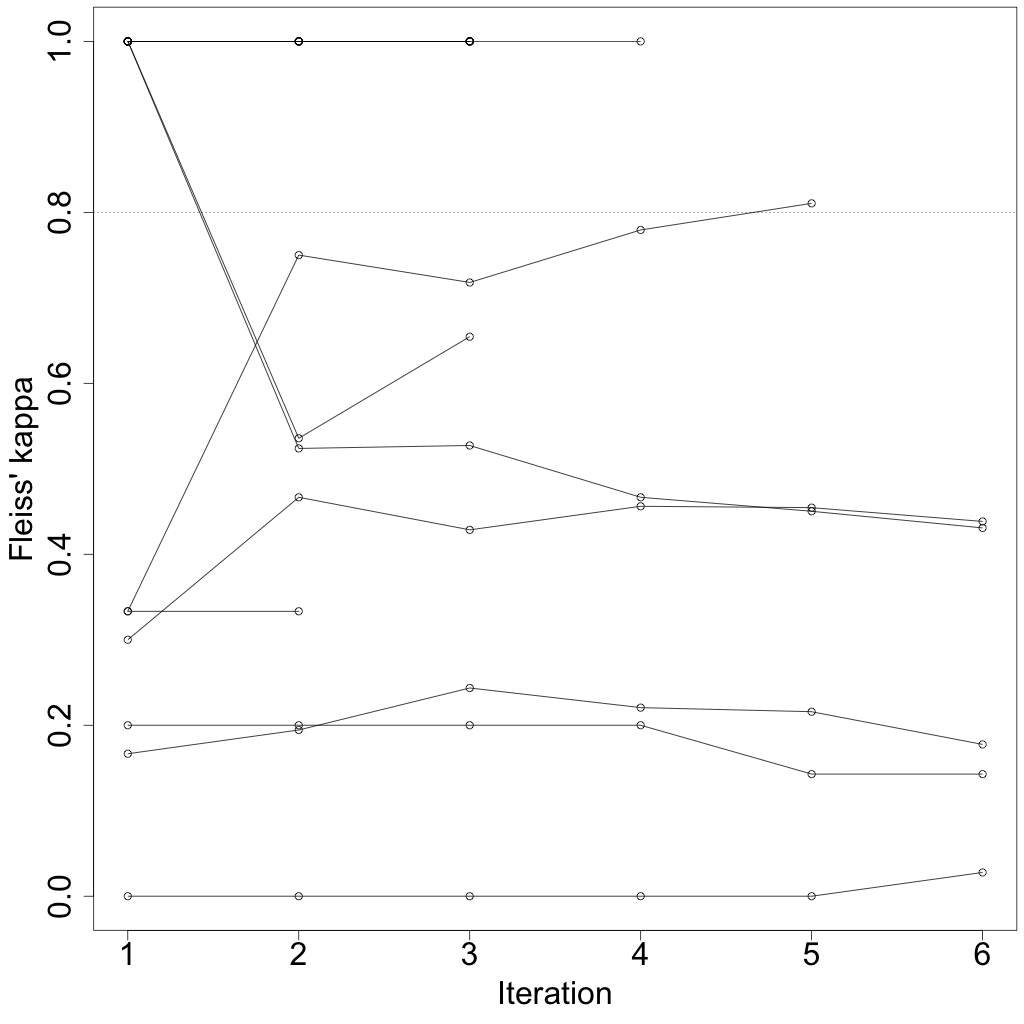
\includegraphics[width=0.49\textwidth]{results-highest-not-found.png}}{\caption{Roads for which the house numbers were not found. Submissions for the highest house number.}\label{fig:results-highest-not-found}}
   \end{floatrow}
\end{figure}
        
\begin{figure}[!ht]
    \begin{floatrow}
        \ffigbox{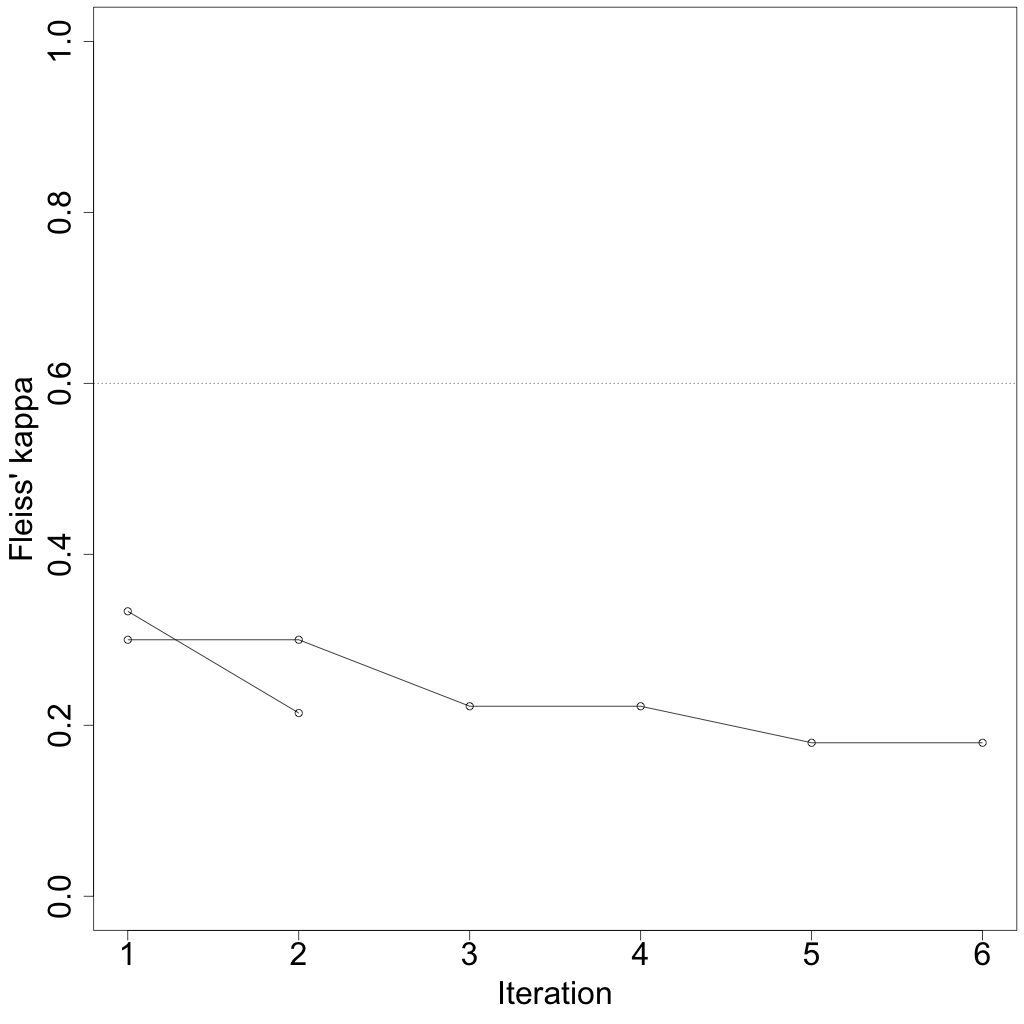
\includegraphics[width=0.49\textwidth]{results-lowest-found.png}}{\caption{Roads for which the house numbers were found. Submissions for the lowest house number.}\label{fig:results-lowest-found}}
        \ffigbox{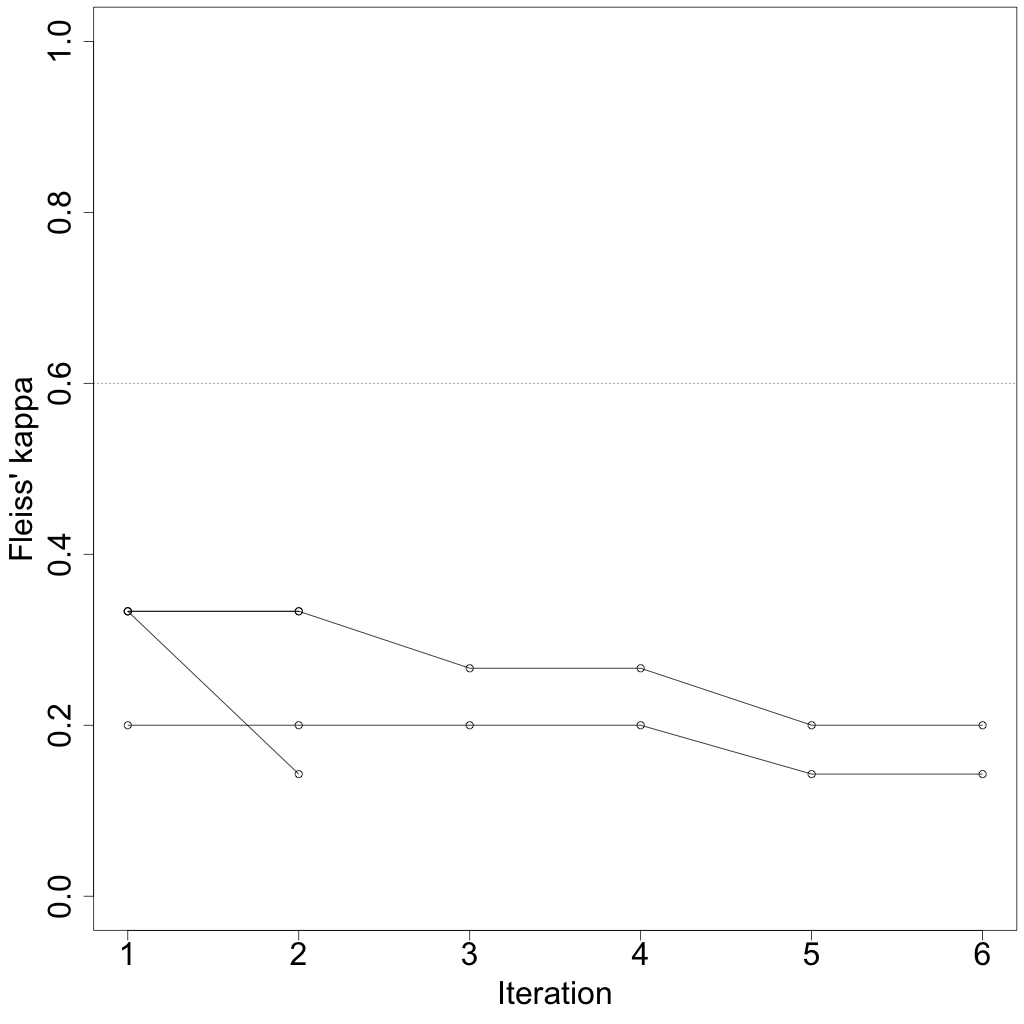
\includegraphics[width=0.49\textwidth]{results-highest-found.png}}{\caption{Roads for which the house numbers were found. Submissions for the highest house number.}\label{fig:results-highest-found}}
   \end{floatrow}
\end{figure}
        
The figures show heterogeneous results, with agreement on several of the roads not only failing to converge, but stalling or worsening with new iterations. 

Cheating is a likeliest cause of consensus failing to achieve high kappa values. When aiming at such a high target, even a single wrong house number submitted by a malicious Worker can substantially negatively impact the metric.

Roads that do not have house numbers are the less problematic. This confirms the hypothesis that consensus would be easier to achieve in that case. This is likely due to the larger proportion of malicious Workers who state that a road offers no house numbers but happen to be correct by chance.

Consensus on roads that do have house numbers is the most difficult to achieve. This may be due to a combination of cheating and sloppy surveying by Workers who are however in good faith. For example, they may be content of finding house numbers that look "small enough" or "high enough". The divergence in submissions for the same road is captured by Fleiss' kappa.